%==============================================================
%  EE201 -- Circuit Theory I
%  Lecture 12 : Mesh Current Analysis
%  M. Mert Ankaralı, METU EEE
%
%  Compile:  ./build.sh      (or: pdflatex EE201_Lecture_12.tex, twice)
%==============================================================
\documentclass[11pt,a4paper]{article}

%-------------------- packages --------------------------------
\usepackage[T1]{fontenc}
\usepackage[utf8]{inputenc}
\usepackage[english]{babel}
\usepackage{lmodern}
\usepackage[margin=2.3cm,top=2.0cm,bottom=1.9cm,headheight=14pt,headsep=9pt]{geometry}
\usepackage{amsmath,amssymb}
\usepackage{array,booktabs,tabularx}
\usepackage{enumitem}
\usepackage{needspace}
\usepackage[table]{xcolor}
\usepackage{fancyhdr}
\usepackage{titlesec}
\usepackage{graphicx}
\usepackage[most]{tcolorbox}
\usepackage{tikz}
\usepackage[american,siunitx]{circuitikz}
\usetikzlibrary{matrix,arrows.meta,positioning,calc,decorations.pathmorphing,decorations.pathreplacing,decorations.markings,patterns,shapes.geometric}
\usepackage[colorlinks=true,allcolors=metured,breaklinks=true]{hyperref}

%-------------------- colour system ---------------------------
% One colour per physical quantity, used identically in the slides.
\definecolor{metured}{RGB}{155,27,48}    % headings, structure
\definecolor{metugray}{RGB}{88,89,91}
\definecolor{ccur}{RGB}{0,102,170}       % CURRENT  -- blue
\definecolor{cvolt}{RGB}{214,120,0}      % VOLTAGE  -- orange
\definecolor{cpow}{RGB}{23,128,74}       % POWER / ENERGY -- green
\definecolor{ccharge}{RGB}{124,60,160}   % CHARGE   -- purple
\definecolor{cflux}{RGB}{0,138,138}      % FLUX -- teal
\definecolor{boxgray}{RGB}{245,245,245}
\definecolor{copper}{RGB}{184,98,30}

\newcommand{\Icol}[1]{\textcolor{ccur}{#1}}
\newcommand{\Vcol}[1]{\textcolor{cvolt}{#1}}
\newcommand{\Pcol}[1]{\textcolor{cpow}{#1}}
\newcommand{\Qcol}[1]{\textcolor{ccharge}{#1}}
\newcommand{\Fcol}[1]{\textcolor{cflux}{#1}}

%-------------------- units (no siunitx dependency) -----------
\newcommand{\uni}[1]{\,\mathrm{#1}}
\newcommand{\A}{\uni{A}}   \newcommand{\V}{\uni{V}}
\newcommand{\W}{\uni{W}}   \newcommand{\J}{\uni{J}}
\newcommand{\Cb}{\uni{C}}  \newcommand{\s}{\uni{s}}
\newcommand{\Sie}{\uni{S}} \newcommand{\Wb}{\uni{Wb}}

%-------------------- layout ----------------------------------
\pagestyle{fancy}
\fancyhf{}
\lhead{\small\textcolor{metugray}{EE201 -- Circuit Theory I}}
\rhead{\small\textcolor{metugray}{Lecture 12: Mesh Current Analysis}}
\cfoot{\small\thepage}
\renewcommand{\headrulewidth}{0.4pt}

\titleformat{\section}{\large\bfseries\color{metured}}{\thesection.}{0.6em}{}
\titleformat{\subsection}{\normalsize\bfseries\color{metugray}}{\thesubsection.}{0.6em}{}
\titlespacing*{\section}{0pt}{1.4ex plus .3ex}{0.7ex}
\titlespacing*{\subsection}{0pt}{1.1ex plus .2ex}{0.5ex}

\setlist[itemize]{itemsep=2pt,topsep=3pt,parsep=0pt,leftmargin=1.5em}
\setlist[enumerate]{itemsep=2pt,topsep=3pt,parsep=0pt,leftmargin=1.7em}
\setlength{\parindent}{0pt}
\setlength{\parskip}{0.7ex plus .1ex}
\raggedbottom
\widowpenalty=10000
\clubpenalty=10000
\brokenpenalty=10000

%-------------------- boxes -----------------------------------
\newtcolorbox{definitionbox}[1]{enhanced,
  colback=metured!4, colframe=metured, boxrule=0.9pt,
  fonttitle=\bfseries, title={#1}, arc=2pt,
  left=7pt,right=7pt,top=5pt,bottom=5pt, before skip=7pt, after skip=7pt,
  before upper={\setlength{\parskip}{0.6ex plus .1ex}}}

\newtcolorbox{ideabox}[1][Key idea]{enhanced,
  colback=ccur!5, colframe=ccur, boxrule=0.9pt,
  fonttitle=\bfseries, title={#1}, arc=2pt,
  left=7pt,right=7pt,top=5pt,bottom=5pt, before skip=7pt, after skip=7pt,
  before upper={\setlength{\parskip}{0.6ex plus .1ex}}}

\newtcolorbox{examplebox}[1][Example]{enhanced,
  colback=cpow!4, colframe=cpow, boxrule=0.9pt,
  fonttitle=\bfseries, title={#1}, arc=2pt,
  left=7pt,right=7pt,top=5pt,bottom=5pt, before skip=7pt, after skip=7pt,
  before upper={\setlength{\parskip}{0.6ex plus .1ex}}}

\newtcolorbox{cautionbox}[1][Careful]{enhanced,
  colback=cvolt!6, colframe=cvolt, boxrule=0.9pt,
  fonttitle=\bfseries, title={#1}, arc=2pt,
  left=7pt,right=7pt,top=5pt,bottom=5pt, before skip=7pt, after skip=7pt,
  before upper={\setlength{\parskip}{0.6ex plus .1ex}}}

%-------------------- circuitikz defaults ---------------------
%  voltage sources: smaller + and - inside the circle, further apart
\ctikzset{bipoles/vsourceam/inner plus={\tiny$+$},
          bipoles/vsourceam/inner minus={\tiny$\vphantom{+}-$},
          bipoles/vsourceam/margin=0.85,
          bipoles/cvsourceam/inner plus={\tiny$+$},
          bipoles/cvsourceam/inner minus={\tiny$\vphantom{+}-$},
          bipoles/cvsourceam/margin=0.85}
\ctikzset{bipoles/length=0.9cm, color=black,
          label/align=straight,
          bipoles/generic/height=0.28, bipoles/generic/width=0.62}
\tikzset{
  iar/.style={-{Stealth[length=2.2mm]}, ccur, thick},
  pol/.style={font=\small, text=cvolt},
  glab/.style={font=\footnotesize, text=metured},
  ttl/.style={font=\scriptsize\bfseries, text=metugray},
  capn/.style={font=\scriptsize, text=metugray, align=center},
  bigarr/.style={-{Stealth[length=3mm]}, very thick, metugray},
  gnode/.style={circle, fill=metured, inner sep=0pt, minimum size=4.4pt},
  nlab/.style={circle, draw=metured, text=metured, font=\scriptsize, inner sep=0.7pt},
  blab/.style={font=\footnotesize, text=black!80},
  gbr/.style={black!75, thick, postaction={decorate, decoration={markings,
      mark=at position 0.56 with {\arrow{Stealth[length=2.5mm]}}}}},
  apbr/.style={ccur, line width=1.7pt, postaction={decorate, decoration={markings,
      mark=at position 0.56 with {\arrow{Stealth[length=2.8mm]}}}}},
  hal/.style={draw=cpow!60, line width=6pt, opacity=0.35, line cap=round, line join=round},
  elem/.style={draw=metugray, thick, fill=metulight},
}
\definecolor{metulight}{RGB}{243,240,241}

%-------------------- Lecture 12 circuit macros ---------------
\newcommand{\ohm}{\,\Omega}
%  Colour-coded matrix entries: diagonal, off-diagonal, right side (#1 = colour of the right side)
\newcommand{\cbx}[2]{{\setlength{\fboxsep}{1.6pt}\colorbox{#1}{$\displaystyle #2\mathstrut$}}}
\newcommand{\dg}[1]{\cbx{cpow!16}{#1}}
\newcommand{\od}[1]{\cbx{metured!13}{#1}}
\newcommand{\chip}[1]{\textcolor{#1}{$\blacksquare$}}

%  An entry that appears on overlay #1, shown in red on that overlay
\newcommand{\zin}[2]{\uncover<#1->{\alt<#1>{{\textcolor{metured}{#2}}}{{#2}}}}
%  A highlighted matrix row entry: colour #1, content #2
\newcommand{\hrow}[2]{{\setlength{\fboxsep}{1.5pt}\colorbox{#1}{\makebox[2.1em]{$\mathstrut #2$}}}}
\newcommand{\yes}{\textcolor{cpow}{\checkmark}}
\newcommand{\no}{\textcolor{metured}{$\boldsymbol{\times}$}}
\newcommand{\e}[1]{\textcolor{cvolt}{e_{#1}}}
\newcommand{\im}[1]{\textcolor{ccur}{i_{M#1}}}
\newcommand{\nd}[1]{\tikz[baseline=(c.base)]\node[nlab](c){#1};}
\tikzset{mlabst/.style={draw=ccur, text=ccur, fill=white, rounded corners=1.5pt,
                        inner sep=1.2pt, font=\scriptsize\bfseries},
         smesh/.style={draw=metured, line width=5pt, opacity=0.28, line join=round}}
%  A boxed mesh number, for the text
\newcommand{\mlab}[1]{\tikz[baseline=(c.base)]\node[mlabst](c){#1};}
\newcommand{\smlab}{\tikz[baseline=(c.base)]\node[nlab](c){S};}
%  A clockwise mesh arrow at (#2,#3) with mesh number #4; optional radius #1
\newcommand{\meshcw}[4][0.36]{%
  \draw[ccur, thick, -{Stealth[length=2mm]}] ($(#2,#3)+(150:#1)$)
    arc[start angle=150, end angle=-150, radius=#1];
  \node[mlabst] at (#2,#3) {#4};}
%  A light disk behind a mesh, to point at it
\newcommand{\meshhalo}[3][0.62]{\fill[ccur!12] (#2,#3) circle (#1);}
\newcommand{\nodev}[3]{\fill (#1) circle (1.7pt) node[#2, inner sep=2pt, font=\small, text=cvolt] {#3};}
\newcommand{\gnd}[2]{\draw (#1,#2) -- ++(0,-0.2) node[ground] {};}

%  Examples 12.1 and 12.2: three meshes.
%  #1 = 0: v_s1 on the left (12.1);  1: i_s on the left (12.2).
%  #2 = 0: no mesh currents;  1: with the clockwise mesh currents.
\newcommand{\exM}[2]{%
  \ifnum#1=0
    \draw (0,2) to[american voltage source, l_=$\Vcol{v_{s1}}$] (0,0);
    \draw (7,0) to[american voltage source, l_=$\Vcol{v_{s2}}$] (7,2);
  \else
    \draw (0,0) to[american current source, l=$\Icol{i_s}$] (0,2);
    \draw (7,0) to[american voltage source, l_=$\Vcol{v_s}$] (7,2);
  \fi
  \draw (0,2) -- (0,3.5) to[R, l=$R_4$] (7,3.5) -- (7,2);
  \draw (0,2) to[R, l=$R_1$] (3.5,2) to[R, l=$R_3$] (7,2);
  \draw (3.5,2) to[R, l=$R_2$] (3.5,0);
  \draw (0,0) -- (7,0);
  \foreach \p in {(0,2),(3.5,2),(7,2),(3.5,0)} \fill \p circle (1.7pt);
  \ifnum#2>0
    \meshcw{1.6}{1.0}{1} \meshcw{5.5}{1.0}{2} \meshcw[0.33]{3.5}{2.8}{3}
  \fi}

%  Examples 12.3 and 12.4: two meshes with a current source between them.
%  #1 = 0: v_s on the right (12.3);  1: the CCVS r_m i_x on the right (12.4).
%  #2 = 0: no mesh currents;  1: mesh currents;  2: mesh currents and the supermesh;
%       3: mesh currents and the voltage v of the current source (Method I).
\newcommand{\exN}[2]{%
  \draw (0,0) to[R, l=$R_1$] (0,2.2) to[R, l=$R_2$] (3,2.2) to[R, l=$R_3$] (6,2.2);
  \draw (3,2.2) to[american current source, l=$\Icol{i_s}$] (3,0);
  \ifnum#1=0
    \draw (6,2.2) to[american voltage source, l=$\Vcol{v_s}$] (6,0);
  \else
    \draw (6,2.2) to[american controlled voltage source, l=$\Vcol{r_m i_x}$] (6,0);
    \draw[iar] (-0.28,1.62) -- (-0.28,2.12); \node[font=\small, text=ccur] at (-0.58,1.9) {$i_x$};
  \fi
  \draw (0,0) -- (6,0);
  \foreach \p in {(3,2.2),(3,0)} \fill \p circle (1.7pt);
  \ifnum#2>0 \meshcw{1.45}{1.1}{1} \meshcw{4.75}{1.1}{2} \fi
  \ifnum#2=2
    \draw[smesh] (0,0) -- (0,2.2) -- (6,2.2) -- (6,0) -- cycle;
    \node[nlab] at (0.55,0.38) {S};
  \fi
  \ifnum#2=3
    \node[pol] at (2.62,1.75) {$+$}; \node[pol] at (2.62,0.45) {$-$};
    \node[font=\small, text=cvolt] at (2.45,1.1) {$v$};
  \fi}

%  Example 12.5: a dependent current source 3 v_x on the top branch.
%  #1 = 0: bare;  1: mesh currents;  2: mesh currents and the supermesh of meshes 1 and 2;
%       3: node voltages (ground at the right node).
\newcommand{\exP}[1]{%
  \draw (7.2,3.8) to[american controlled current source, l_=$\Icol{3\,v_x}$] (0,3.8);
  \draw (0,3.8) -- (0,2); \draw (7.2,3.8) -- (7.2,2);
  \draw (0,2) to[R, l=$4\ohm$] (3.6,2) to[american voltage source, l=$\Vcol{12\V}$] (7.2,2);
  \draw (0,0) to[R, l=$2\ohm$] (0,2);
  \draw (3.6,0) to[american current source, l_=$\Icol{2\A}$] (3.6,2);
  \draw (7.2,2) to[R, l=$6\ohm$] (7.2,0);
  \draw (0,0) -- (7.2,0);
  \foreach \p in {(0,2),(3.6,2),(7.2,2),(3.6,0)} \fill \p circle (1.7pt);
  \node[pol] at (0.35,1.6) {$+$}; \node[pol] at (0.35,0.4) {$-$};
  \node[font=\small, text=cvolt] at (0.5,1.0) {$v_x$};
  \draw[iar] (1.45,1.72) -- (2.15,1.72); \node[font=\small, text=ccur] at (2.4,1.72) {$i$};
  \ifnum#1>0 \ifnum#1<3
    \meshcw{1.65}{0.85}{1} \meshcw{5.7}{0.9}{2} \meshcw[0.32]{3.6}{2.95}{3}
  \fi\fi
  \ifnum#1=2
    \draw[smesh] (0,0) -- (0,2) -- (7.2,2) -- (7.2,0) -- cycle;
    \node[nlab] at (3.1,0.35) {S};
  \fi
  \ifnum#1=3
    \node[font=\small, text=cvolt, anchor=south east] at (-0.05,2.05) {$e_1$};
    \node[font=\small, text=cvolt, anchor=north] at (3.6,-0.1) {$e_2$};
    \draw (7.2,3.8) -- (7.8,3.8) -- (7.8,3.6) node[ground] {};
  \fi}

%  Example 12.5: a dependent voltage source 2 i_x on the right branch.
%  #1 = 0: bare;  1: mesh currents.
\newcommand{\exQ}[1]{%
  \draw (0,2.2) to[american voltage source, l_=$\Vcol{16\V}$] (0,0);
  \draw (0,2.2) to[R, l=$2\ohm$] (3.5,2.2) to[R, l=$2\ohm$] (7,2.2);
  \draw (3.5,2.2) to[R, l=$4\ohm$] (3.5,0);
  \draw (7,2.2) to[american controlled voltage source, l=$\Vcol{2\,i_x}$] (7,0);
  \draw (0,0) -- (7,0);
  \foreach \p in {(3.5,2.2),(3.5,0)} \fill \p circle (1.7pt);
  \draw[iar] (3.12,1.45) -- (3.12,0.75); \node[font=\small, text=ccur, anchor=east] at (3.07,1.1) {$i_x$};
  \ifnum#1>0 \meshcw{1.55}{1.1}{1} \meshcw{5.25}{1.1}{2} \fi}

%  Graph branch from #2 to #3, label #5 on side #4 (angle), optional colour #1
\newcommand{\gbranch}[5][black!75]{%
  \draw[gbr, #1] (#2) -- (#3);
  \node[blab, text=#1] at ($(#2)!0.5!(#3)!0.3cm!#4:(#3)$) {#5};}
%  The graph of Example 12.1: branches 1-4 the resistors R1-R4, 5 and 6 the sources v_s1, v_s2.
%  #1 = 0: graph only;  1: with the clockwise meshes.
\newcommand{\exMgraph}[1]{%
  \coordinate (ga) at (0,1.5); \coordinate (gb) at (2.2,1.5);
  \coordinate (gc) at (4.4,1.5); \coordinate (gd) at (2.2,0);
  \gbranch{ga}{gb}{90}{1}
  \gbranch{gb}{gd}{0}{2}
  \gbranch{gb}{gc}{90}{3}
  \draw[gbr] (ga) to[bend left=50] (gc); \node[blab] at (2.2,2.72) {4};
  \draw[gbr, cvolt] (ga) to[bend right=40] (gd); \node[blab, text=cvolt] at (0.42,0.32) {5};
  \draw[gbr, cvolt] (gd) to[bend right=40] (gc); \node[blab, text=cvolt] at (3.98,0.32) {6};
  \foreach \k in {a,b,c,d} \fill[metured] (g\k) circle (2.2pt);
  \ifnum#1>0
    \meshcw[0.27]{1.3}{0.82}{1} \meshcw[0.27]{3.1}{0.82}{2} \meshcw[0.27]{2.2}{2.08}{3}
  \fi}
%  A mesh matrix with mesh labels on the left and branch numbers on top.
%  #1 name, #2 number of columns, #3 number of rows, #4 rows (entries separated by \&), #5 extra TikZ
\newcommand{\meshmat}[5]{%
  \begin{tikzpicture}[baseline={([yshift=-0.6ex]#1.center)}]
    \matrix (#1) [matrix of math nodes, ampersand replacement=\&,
                  left delimiter={[}, right delimiter={]}, inner sep=1pt,
                  column sep=0.45em,
                  nodes={text width=1.35em, align=right, minimum height=1.25em,
                         inner sep=1pt}] {#4};
    \foreach \j in {1,...,#2}
      \node[font=\scriptsize, text=metugray, anchor=south east, inner sep=1pt]
        at ([yshift=2pt]#1-1-\j.north east) {\j};
    \foreach \i in {1,...,#3}
      \node[mlabst, left=11pt] at (#1.west |- #1-\i-1) {\i};
    #5
  \end{tikzpicture}}
%  \exMmatN{k}: the mesh matrix M of Example 12.1 with its first k rows filled in;
%  k = 4 adds the M_R / M_S boxes
\newcommand{\phrow}{\phantom{0} \& \phantom{0} \& \phantom{0} \& \phantom{0} \& \phantom{0} \& \phantom{0}}
\newcommand{\exMmatN}[1]{%
  \ifnum#1>0 \def\rowA{1 \& 1 \& 0 \& 0 \& \textcolor{cvolt}{-1} \& \textcolor{cvolt}{0}}%
  \else\let\rowA\phrow\fi
  \ifnum#1>1 \def\rowB{0 \& -1 \& 1 \& 0 \& \textcolor{cvolt}{0} \& \textcolor{cvolt}{-1}}%
  \else\let\rowB\phrow\fi
  \ifnum#1>2 \def\rowC{-1 \& 0 \& -1 \& 1 \& \textcolor{cvolt}{0} \& \textcolor{cvolt}{0}}%
  \else\let\rowC\phrow\fi
  \meshmat{MM}{6}{3}{\rowA\\ \rowB\\ \rowC\\}{%
    \ifnum#1>3
    \draw[metugray, thick, rounded corners=2pt]
      ([xshift=-2pt, yshift=1pt]MM-1-1.north west) rectangle ([xshift=2pt, yshift=-1pt]MM-3-4.south east);
    \draw[cvolt, thick, rounded corners=2pt]
      ([xshift=-2pt, yshift=1pt]MM-1-5.north west) rectangle ([xshift=2pt, yshift=-1pt]MM-3-6.south east);
    \node[font=\small, text=metugray, below=3pt] at ($(MM-3-1.south)!0.5!(MM-3-4.south)$) {$M_R$: resistors};
    \node[font=\small, text=cvolt, below=3pt] at ($(MM-3-5.south)!0.5!(MM-3-6.south)$) {$M_S$: sources};
    \else
    \node[font=\small, below=3pt] at ($(MM-3-1.south)!0.5!(MM-3-4.south)$) {\phantom{$M_R$: resistors}};
    \fi}}
\newcommand{\exMmat}{\exMmatN{4}}
\begin{document}

%-------------------- title block -----------------------------
\begin{center}
\begin{tcolorbox}[enhanced, colback=metured!5, colframe=metured, boxrule=1pt,
                  arc=3pt, left=10pt,right=10pt,top=7pt,bottom=7pt, width=\textwidth]
\begin{center}
  {\small\scshape Middle East Technical University}\\[2pt]
  {\small\scshape Department of Electrical and Electronics Engineering}\\[7pt]
  {\Large\bfseries\color{metured} EE201 -- Circuit Theory I}\\[4pt]
  {\large\bfseries Lecture 12: Mesh Current Analysis}\\[6pt]
  {\small M. Mert Ankaralı}
\end{center}
\end{tcolorbox}
\end{center}
\vspace{-0.5em}

\begin{center}
\small
\begin{tabular}{@{}l l@{}}
\toprule
\multicolumn{2}{@{}l}{\textbf{Colour code used in these notes and in the slides}}\\
\midrule
\Icol{$\blacksquare$}~current $i$, mesh current $\im{k}$ around mesh \mlab{k} \quad
\Vcol{$\blacksquare$}~voltage $v$, node voltage $e$ &
\textcolor{metured}{$\blacksquare$}~supermesh \nd{S}\\
\bottomrule
\end{tabular}
\end{center}

\textbf{Motivation.} Node voltage analysis takes the $n - 1$ node voltages as the unknowns.
Then KVL holds automatically, and we write KCL. \textbf{Mesh current analysis} does the
opposite. Its unknowns are the $\ell = b - n + 1$ mesh currents. Every branch current is
$\Icol{\mathbf{i}} = M^T\Icol{\mathbf{i}_M}$, so KCL holds automatically (previously), and we
write KVL around each inner mesh. Meshes need a planar circuit: one drawn with no crossing
branches.

%==============================================================
\section{The procedure, on an example}

For now, the circuit has only resistors and independent voltage sources; current sources and
dependent sources come later. The circuit of Example 12.1 has $b = 6$ branches, so $12$ branch
voltages and currents. Mesh current analysis needs only $3$ unknowns. Four steps find them.

\begin{examplebox}[Example 12.1 --- mesh current analysis step by step]
\begin{minipage}[c]{0.42\linewidth}
\centering
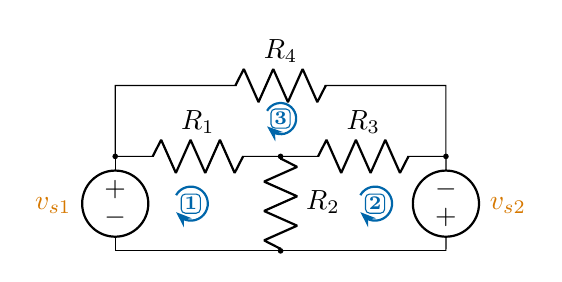
\begin{tikzpicture}[scale=0.6]
  \exM{0}{1}
\end{tikzpicture}
\end{minipage}\hfill
\begin{minipage}[c]{0.56\linewidth}
\begin{enumerate}
  \item \textbf{Inner meshes.} The circuit is planar; its windows are the inner meshes,
        $\ell = 6 - 4 + 1 = 3$.
  \item \textbf{Mesh currents.} Give each a clockwise mesh current $\im{1}$, $\im{2}$, $\im{3}$.
        Every branch current is a combination of them ($\Icol{i_{R_2}} = \im{1} - \im{2}$
        downwards), so KCL holds automatically.
  \item \textbf{Voltages.} Along mesh $k$, a resistor $R$ shared with mesh $j$ has the voltage
        $R(\im{k} - \im{j})$; on mesh $k$ only, $R\,\im{k}$.
  \item \textbf{KVL} around every inner mesh:
\end{enumerate}
\end{minipage}
\begin{alignat*}{2}
  &\text{mesh 1:}\qquad & -\Vcol{v_{s1}} + R_1(\im{1} - \im{3}) + R_2(\im{1} - \im{2}) &= 0\\
  &\text{mesh 2:}\qquad & R_2(\im{2} - \im{1}) + R_3(\im{2} - \im{3}) - \Vcol{v_{s2}} &= 0\\
  &\text{mesh 3:}\qquad & R_4\,\im{3} + R_3(\im{3} - \im{2}) + R_1(\im{3} - \im{1}) &= 0
\end{alignat*}
Mesh 1 meets $\Vcol{v_{s1}}$ from $-$ to $+$, so it enters with a minus sign. Three equations,
three unknowns; then Steps 2 and 3 give every branch current and voltage.
\end{examplebox}

In general, $\Icol{\mathbf{i}} = M^T\Icol{\mathbf{i}_M}$ (KCL holds automatically), the element
laws give $\Vcol{\mathbf{v}}$, and KVL $M\Vcol{\mathbf{v}} = \mathbf{0}$ gives $\ell$ equations
in the $\ell$ mesh currents.

%==============================================================
\section{Matrix form}

With all mesh currents clockwise, the three equations of Example 12.1 become
\[
  \underbrace{\begin{bmatrix}
    \dg{R_1 + R_2} & \od{-R_2} & \od{-R_1}\\[2pt]
    \od{-R_2} & \dg{R_2 + R_3} & \od{-R_3}\\[2pt]
    \od{-R_1} & \od{-R_3} & \dg{R_1 + R_3 + R_4}
  \end{bmatrix}}_{Z_M}
  \underbrace{\begin{bmatrix} \im{1}\\[2pt] \im{2}\\[2pt] \im{3} \end{bmatrix}}_{\Icol{\mathbf{i}_M}}
  =
  \underbrace{\begin{bmatrix} \cbx{cvolt!16}{\Vcol{v_{s1}}}\\[2pt] \cbx{cvolt!16}{\Vcol{v_{s2}}}\\[2pt] \cbx{cvolt!16}{0} \end{bmatrix}}_{\Vcol{\mathbf{v}_M}} .
\]
$Z_M$ is the \textbf{mesh impedance matrix}, and $Z_M\Icol{\mathbf{i}_M} = \Vcol{\mathbf{v}_M}$
are the \textbf{mesh equations}; $\Vcol{\mathbf{v}_M}$ holds the source voltages rising along
each mesh. The three colours follow three rules, so for a circuit of resistors and voltage
sources the mesh equations can be written down directly.

\begin{ideabox}[Writing $Z_M$ directly from the circuit: three rules]
\begin{itemize}
  \item \chip{cpow!45} \textbf{Diagonal} entry $(k,k)$: the sum of the resistances around mesh $k$.
  \item \chip{metured!50} \textbf{Off-diagonal} entry $(k,j)$: minus the sum of the resistances shared by meshes $k$ and $j$.
  \item \chip{cvolt!50} \textbf{Right side}, row $k$: the sum of the source voltages rising (met from $-$ to $+$) along mesh $k$.
\end{itemize}
In Example 12.1:
\par\smallskip
{\centering\small
\renewcommand{\arraystretch}{1.15}
\begin{tabular}{@{}lll@{}}
  \cellcolor{cpow!16}\textbf{Diagonal} & \cellcolor{metured!13}\textbf{Off-diagonal} & \cellcolor{cvolt!16}\textbf{Right side}\\
  $(1,1)$: $R_1, R_2$ around mesh 1 & $(1,2)$, $(2,1)$: $R_2$ shared by 1 and 2 & row 1: $\Vcol{v_{s1}}$ rises along mesh 1\\
  $(2,2)$: $R_2, R_3$ around mesh 2 & $(1,3)$, $(3,1)$: $R_1$ shared by 1 and 3 & row 2: $\Vcol{v_{s2}}$ rises along mesh 2\\
  $(3,3)$: $R_1, R_3, R_4$ around mesh 3 & $(2,3)$, $(3,2)$: $R_3$ shared by 2 and 3 & row 3: no source
\end{tabular}\par}
\smallskip
Each shared resistance appears twice, at $(k,j)$ and $(j,k)$: $Z_M$ is \textbf{symmetric}.
\end{ideabox}

\textbf{$Z_M$ from the graph.} In the graph of Example 12.1, branches 1--4 are the resistors
$R_1, \dots, R_4$, and branches 5 and 6 are the sources $\Vcol{v_{s1}}$, $\Vcol{v_{s2}}$; a
source branch points from $+$ to $-$. The mesh matrix $M$ has one row for each inner mesh; an
entry is $+1$ if the branch goes along the mesh and $-1$ if against it.

\begin{center}
\begin{minipage}[c]{0.36\linewidth}
\centering
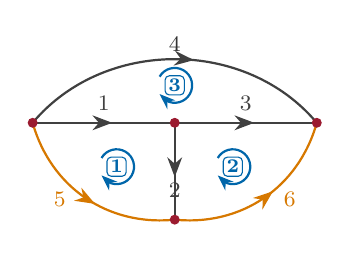
\begin{tikzpicture}[scale=0.82]
  \exMgraph{1}
\end{tikzpicture}
\end{minipage}%
\begin{minipage}[c]{0.6\linewidth}
\centering
$M = \exMmat$
\end{minipage}
\end{center}

KVL $M\Vcol{\mathbf{v}} = \mathbf{0}$ reads $M_R\Vcol{\mathbf{v}_R} + M_S\Vcol{\mathbf{v}_S} = \mathbf{0}$.
The resistors obey $\Vcol{\mathbf{v}_R} = R\,\Icol{\mathbf{i}_R}$ with
$R = \mathrm{diag}(R_1, \dots, R_4)$. KCL, $\Icol{\mathbf{i}} = M^T\Icol{\mathbf{i}_M}$, splits into
rows: $\left[\begin{smallmatrix} \Icol{\mathbf{i}_R}\\ \Icol{\mathbf{i}_S} \end{smallmatrix}\right]
= \left[\begin{smallmatrix} M_R^T\\ M_S^T \end{smallmatrix}\right]\Icol{\mathbf{i}_M}$, so
$\Icol{\mathbf{i}_R} = M_R^T\Icol{\mathbf{i}_M}$ (resistor rows) and
$\Icol{\mathbf{i}_S} = M_S^T\Icol{\mathbf{i}_M}$ (source rows); only the resistor rows are
needed. In Example 12.1, $M_R^T$ is the resistor columns 1--4 of $M$ written
as rows, and
\[
  \Icol{\mathbf{i}_R} = M_R^T\Icol{\mathbf{i}_M} =
  \begin{bmatrix} 1 & 0 & -1\\ 1 & -1 & 0\\ 0 & 1 & -1\\ 0 & 0 & 1 \end{bmatrix}
  \begin{bmatrix} \im{1}\\ \im{2}\\ \im{3} \end{bmatrix}
  = \big[\, \im{1} - \im{3} \quad \im{1} - \im{2} \quad \im{2} - \im{3} \quad \im{3} \,\big]^T :
\]
each resistor current is the mesh currents along its arrow minus those against it. Together,
\[
  M_R\, R\, M_R^T\,\Icol{\mathbf{i}_M} = -M_S\Vcol{\mathbf{v}_S}
  \quad\Rightarrow\quad
  Z_M = M_R\, R\, M_R^T, \qquad \Vcol{\mathbf{v}_M} = -M_S\Vcol{\mathbf{v}_S}.
\]
For Example 12.1,
\[
  M_R\, R = \begin{bmatrix}
    R_1 & R_2 & 0 & 0\\ 0 & -R_2 & R_3 & 0\\ -R_1 & 0 & -R_3 & R_4
  \end{bmatrix}, \qquad
  -M_S\Vcol{\mathbf{v}_S} = -\begin{bmatrix} -1 & 0\\ 0 & -1\\ 0 & 0 \end{bmatrix}
  \begin{bmatrix} \Vcol{v_{s1}}\\ \Vcol{v_{s2}} \end{bmatrix}
  = \begin{bmatrix} \Vcol{v_{s1}}\\ \Vcol{v_{s2}}\\ 0 \end{bmatrix},
\]
and $M_R\, R\, M_R^T$ is exactly the $Z_M$ above: the three rules read this product off entry by
entry. Finally, $Z_M^T = M_R R^T M_R^T = Z_M$, since $R$ is diagonal: with resistors and voltage
sources, $Z_M$ is always symmetric.

%==============================================================
\section{A current source on one mesh only}

\begin{definitionbox}{A current source on one mesh only}
If an independent current source $\Icol{i_s}$ is on mesh $k$ only (on the outer boundary), then
$\im{k} = \pm\Icol{i_s}$ is known. So $\im{k}$ is not an unknown, and KVL is not written around
mesh $k$: the voltage of the current source is not known.
\end{definitionbox}

\begin{examplebox}[Example 12.2 --- a current source on mesh 1]
\begin{minipage}[c]{0.37\linewidth}
\centering
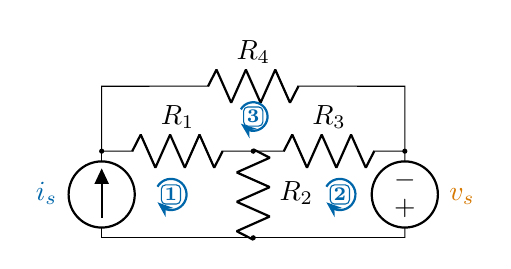
\begin{tikzpicture}[scale=0.55]
  \exM{1}{1}
\end{tikzpicture}
\end{minipage}\hfill
\begin{minipage}[c]{0.61\linewidth}
The source $\Icol{i_s}$ points along mesh 1, so $\im{1} = \Icol{i_s}$; the unknowns are only
$\im{2}$, $\im{3}$.
\begin{align*}
  \text{mesh 2:}\quad & R_2(\im{2} - \Icol{i_s}) + R_3(\im{2} - \im{3}) - \Vcol{v_s} = 0\\
  \text{mesh 3:}\quad & R_1(\im{3} - \Icol{i_s}) + R_3(\im{3} - \im{2}) + R_4\,\im{3} = 0
\end{align*}
\end{minipage}
\end{examplebox}
In matrix form, Example 12.2 reads
\[
  \begin{bmatrix} R_2 + R_3 & -R_3\\ -R_3 & R_1 + R_3 + R_4 \end{bmatrix}
  \begin{bmatrix} \im{2}\\ \im{3} \end{bmatrix}
  = \begin{bmatrix} \Vcol{v_s} + R_2\Icol{i_s}\\ R_1\Icol{i_s} \end{bmatrix} .
\]
The known $\Icol{i_s}$ moves to the right side: $R_2\Icol{i_s}$ acts like a source voltage on mesh 2.

%==============================================================
\section{A current source between two meshes: modified mesh analysis}

If a current source (independent or dependent) is shared by two meshes, KVL around either mesh
needs its voltage, but its voltage cannot be written with mesh currents. Its law fixes its
current, not its voltage. \textbf{Modified mesh current analysis} offers two ways out.

\begin{definitionbox}{Method I}
Let the unknown voltage $\Vcol{v}$ of the current source be one more unknown. Write KVL around
every inner mesh, and add the law of the source as a \textbf{constraint equation}.
\end{definitionbox}

\begin{examplebox}[Example 12.3 --- Method I]
\begin{minipage}[c]{0.4\linewidth}
\centering
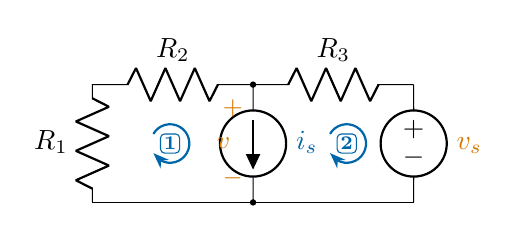
\begin{tikzpicture}[scale=0.68]
  \exN{0}{3}
\end{tikzpicture}
\end{minipage}\hfill
\begin{minipage}[c]{0.58\linewidth}
\begin{align*}
  \text{mesh 1:}\quad & (R_1 + R_2)\,\im{1} + \Vcol{v} = 0\\
  \text{mesh 2:}\quad & R_3\,\im{2} + \Vcol{v_s} - \Vcol{v} = 0\\
  \text{constraint:}\quad & \im{1} - \im{2} = \Icol{i_s}
\end{align*}
\end{minipage}
\[
  \begin{bmatrix}
    R_1 + R_2 & 0 & 1\\ 0 & R_3 & -1\\ 1 & -1 & 0
  \end{bmatrix}
  \begin{bmatrix} \im{1}\\ \im{2}\\ \Vcol{v} \end{bmatrix}
  = \begin{bmatrix} 0\\ -\Vcol{v_s}\\ \Icol{i_s} \end{bmatrix}
\]
Three unknowns and three equations; the last row is the constraint.
\end{examplebox}

\textbf{Method II: the supermesh.} Add the KVL equations of meshes 1 and 2: $\Vcol{v}$ enters
mesh 1 with $+$ and mesh 2 with $-$, so it cancels. The sum is KVL around the outer loop of the
two meshes, which avoids the current source.

\begin{definitionbox}{Method II: the supermesh}
Write KVL around two meshes as if they were a single mesh, skipping the current source between
them. Such a loop is a \textbf{supermesh}. Add the law of the source as a constraint equation.
\end{definitionbox}

\textbf{Example 12.3, revisited with a supermesh} (circuit above, the loop \nd{S} around meshes
1 and 2): the unknowns are $\im{1}$, $\im{2}$, and
\[
  \left.
  \begin{aligned}
    \text{supermesh:}\quad & (R_1 + R_2)\,\im{1} + R_3\,\im{2} + \Vcol{v_s} = 0\\
    \text{constraint:}\quad & \im{1} - \im{2} = \Icol{i_s}
  \end{aligned}
  \ \right\}
  \quad\Rightarrow\quad
  \begin{bmatrix} R_1 + R_2 & R_3\\ 1 & -1 \end{bmatrix}
  \begin{bmatrix} \im{1}\\ \im{2} \end{bmatrix}
  = \begin{bmatrix} -\Vcol{v_s}\\ \Icol{i_s} \end{bmatrix} .
\]
Method II has one unknown fewer than Method I and gives the same mesh currents; in both, the
matrix is no longer symmetric.

%==============================================================
\section{Dependent sources}

A dependent source is handled like an independent one of the same kind. Its control variable is
then written with mesh currents. First plug it into the equations, then form the matrix.

\begin{examplebox}[Example 12.4 --- a dependent current source]
\begin{minipage}[c]{0.44\linewidth}
\centering
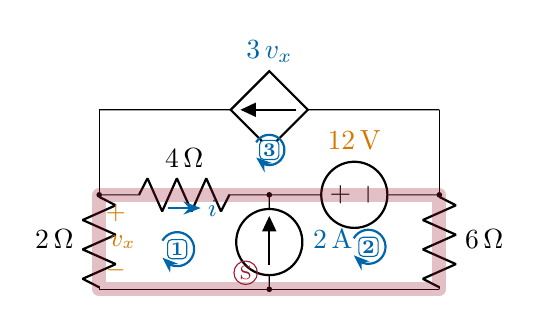
\begin{tikzpicture}[scale=0.6]
  \exP{2}
\end{tikzpicture}
\end{minipage}\hfill
\begin{minipage}[c]{0.54\linewidth}
\textbf{Question.} Find $\Icol{i}$, the current of the $4\ohm$.

\textbf{Answer.} The $2\A$ source is between meshes 1 and 2: use the supermesh \nd{S}. The
dependent source is on mesh 3 only: it fixes $\im{3}$. So KVL is written around \nd{S} only:
\[
  2\,\im{1} + 4(\im{1} - \im{3}) + 12 + 6\,\im{2} = 0 \qquad (1)
\]
\end{minipage}

\smallskip
The $2\A$ source gives $\im{2} - \im{1} = 2$ (2). The dependent source gives
$\im{3} = -3\,\Vcol{v_x}$; $\im{1}$ flows up through the $2\ohm$, from $-$ to $+$, so
$\Vcol{v_x} = -2\,\im{1}$ and $\im{3} = 6\,\im{1}$ (3). In matrix form,
\[
  \begin{bmatrix} 6 & 6 & -4\\ -1 & 1 & 0\\ -6 & 0 & 1 \end{bmatrix}
  \begin{bmatrix} \im{1}\\ \im{2}\\ \im{3} \end{bmatrix}
  = \begin{bmatrix} -12\\ 2\\ 0 \end{bmatrix}
  \quad\Rightarrow\quad \im{1} = 2\A,\ \ \im{2} = 4\A,\ \ \im{3} = 12\A,
\]
so $\Icol{i} = \im{1} - \im{3} = 2 - 12 = \Icol{-10\A}$.
\end{examplebox}

\begin{examplebox}[Example 12.5 --- a dependent voltage source]
\begin{minipage}[c]{0.44\linewidth}
\centering
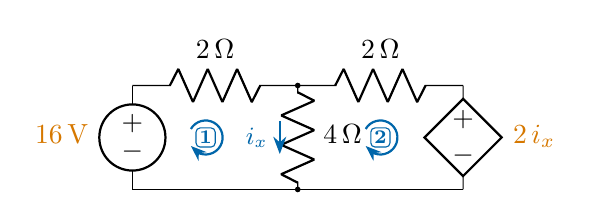
\begin{tikzpicture}[scale=0.6]
  \exQ{1}
\end{tikzpicture}
\end{minipage}\hfill
\begin{minipage}[c]{0.54\linewidth}
\textbf{Question.} Find $\Icol{i_x}$. Treat $\Vcol{2\,i_x}$ as a voltage source:
\begin{alignat*}{2}
  &\text{mesh 1:}\ \ & -16 + 2\,\im{1} + 4(\im{1} - \im{2}) &= 0\\
  &\text{mesh 2:}\ \ & 4(\im{2} - \im{1}) + 2\,\im{2} + \Vcol{2\,i_x} &= 0
\end{alignat*}
First plug $\Icol{i_x} = \im{1} - \im{2}$ into mesh 2: $-2\,\im{1} + 4\,\im{2} = 0$.
Then the matrix:
\[
  \begin{bmatrix} 6 & -4\\ -2 & 4 \end{bmatrix}
  \begin{bmatrix} \im{1}\\ \im{2} \end{bmatrix}
  = \begin{bmatrix} 16\\ 0 \end{bmatrix}
  \ \Rightarrow\ \begin{array}{l} \im{1} = 4\A\\ \im{2} = 2\A \end{array}
\]
So $\Icol{i_x} = 4 - 2 = \Icol{2\A}$. $Z_M$ is not symmetric.
\end{minipage}
\end{examplebox}

\begin{definitionbox}{Remark: a dependent current source on one mesh only}
If a dependent current source is on mesh $k$ only, do not write KVL around mesh $k$: its voltage
is not known. Write its constraint instead.
\end{definitionbox}

%==============================================================
\section{Node or mesh?}

Which method needs fewer equations for Example 12.4? With mesh currents, $\ell = 3$ and each
current source fixes one unknown: $3 - 2 = 1$ KVL equation is left. With node voltages,
$n - 1 = 3$ and each voltage source fixes one: $3 - 1 = 2$ KCL equations are left.

\textbf{Tip.} Count before you start: for mesh currents, $\ell$ minus the current sources; for
node voltages, $n - 1$ minus the voltage sources. Mesh current analysis needs a planar circuit;
node voltage analysis always works.

%==============================================================
\section*{Summary}

\begin{center}
\small
\renewcommand{\arraystretch}{1.15}
\begin{tabular}{@{}>{\raggedright}p{5.4cm} >{\raggedright\arraybackslash}p{10.3cm}@{}}
\toprule
\textbf{In the circuit} & \textbf{What to do}\\
\midrule
resistors and voltage sources & KVL around every inner mesh: $Z_M\Icol{\mathbf{i}_M} =
  \Vcol{\mathbf{v}_M}$, from three simple rules; $Z_M = M_R R M_R^T$ is symmetric\\
a current source on one mesh only & $\im{k}$ is known; no KVL around mesh $k$\\
a current source between meshes & Method I: its voltage as an unknown, plus the
  constraint;\newline Method II: KVL around the supermesh, plus the constraint\\
a dependent source & write its control variable with mesh currents: a constraint equation\\
node or mesh? & count the equations left; mesh current analysis needs a planar circuit\\
\bottomrule
\end{tabular}
\end{center}
After the mesh currents are found: $\Icol{\mathbf{i}} = M^T\Icol{\mathbf{i}_M}$, then the
branch voltages from the element laws.

\end{document}
